\documentclass[10pt,a4paper]{book}
\usepackage[utf8]{inputenc}
\usepackage[english]{babel}
\usepackage{amsmath}
\usepackage{amsfonts}
\usepackage{amssymb}
\usepackage{graphicx}
\usepackage[left=2cm,right=2cm,top=2cm,bottom=2cm]{geometry}

% Thesis title
%\title{Energy Efficiency, Exascale and Complex Systems}
\title{Vers l'Exascale: Des Probl\`emes Th\'eoriques aux Probl\`emes Appliqu\'es\\
The Way to Exascale: From Theorics to Applied Problems}
% Author
\author{Julien Loiseau}
% Date 
\date{\today}

\makeindex

\begin{document}

\thispagestyle{empty}

{%%%
\sffamily
\centering

{
\includegraphics[scale=1]{figures/style/logo_urca_front_page.jpg}
\vspace{0.5cm}
}

{
UNIVERSIT\'E DE REIMS CHAMPAGNE-ARDENNE\\
\vspace{0.5cm}
INFORMATIQUE\\
\vspace{0.5cm}
\'Ecole Doctorale Sciences Technologie Sant\'e
}

\vspace{1.0cm}
{\hrule height 2pt\vspace{2pt}}

\Large

% Title 
{\huge 
\vspace{1cm}
The Way to Exascale: From Theorics to Applied Problems
}

% Subtitle 
{
\vspace{0.5cm}
Vers l'Exascale: Des Probl\`emes Th\'eoriques aux Probl\`emes Appliqu\'es\\
}

\vspace{1.0cm}
\hrule

\vspace{2.5cm}

{\LARGE
par \textbf{Julien Loiseau}
}

\vspace{2.5cm}

{
Th\`ese de doctorat d'Informatique
}

\vspace{2.5cm}

{
Sous la direction de : \textbf{M. Michaël KRAJECKI, Professeur des Universités}
}
\vspace{0.5cm}

\vspace{\fill}

{\normalsize
\begin{tabular}{l l l}
\textbf{JURY} &  & \\
&&\\
?? & ?? & Rapporteur\\
?? & ?? & Rapporteur\\
Benjamin Bergen & Docteur-Ingénieur au Los Alamos National Laboratory, USA & Examinateur \\
Guillaume Colin de Verdière & Ingénieur au CEA & Examinateur\\
Michaël KRAJECKI & Professeur à l'Université de Reims Champagne-Ardenne & Directeur \\
Christophe JAILLET & Maître de Conférence à l'Université de Reims Champagne-Ardenne & Co-directeur \\
François ALIN & Maître de Conférence à l'Université de Reims Champagne-Ardenne & Encadrant \\
\end{tabular}

\vspace{0.5cm}

\hrule

\vspace{0.5cm}

Centre de Recherche en STIC équipe CASH

}

%%%
}%%%

% Empty page after title 
\thispagestyle{empty}

% Setup numbering for beginning 
\frontmatter

% Acknoledgments, thanks everybody !
\addcontentsline{toc}{chapter}{Acknowledgements}
\chapter*{Acknoledgments}

Croyez ceux qui cherchent la vérité, doutez de ceux qui la trouvent; doutez de tout, mais ne doutez pas de vous-même.

% Add the tableofcontentes in itself
\addcontentsline{toc}{chapter}{Contents}
\tableofcontents

% Table of figures
\addcontentsline{toc}{chapter}{List of Figures}
\listoffigures

% Table of tables
\addcontentsline{toc}{chapter}{List of Tables}
\listoftables

\mainmatter
% Introduction
\addcontentsline{toc}{chapter}{Introduction}
\chapter*{Introduction}

In the aurora 2020-2021 for United States of America and maybe before, like 2019 for China, the world of High Performance Computing (HPC) will reach another milestone in the power of machines: the Exascale. 
These supercomputers will be $100$ times faster than the estimated overfall operations performed by the human brain and its $10^{16}$ \textbf{FL}oating point \textbf{O}perations \textbf{P}er \textbf{S}econd (FLOPS) and achieve a computational power of a trillion ($10^{18}$) FLOPS.
This odyssey started long time ago with the first vacuum tubes computers and the need of balistic computation in war. 
Nowdays the main aim is very nearby and the power of a nation is represented by its army and money but also by the computational power of its supercomputers but the HPC's applications also spread into all the area of science and technology.\\

Since 1962, considering the Cray CDC 6600 as the first supercomputer, the power of those machines have increase following an observation of the co-fonder of the Intel company, Gordon Moore. 
Better known under the name of "Moore's Law", it speculates in 1965 that: considering the constant evoluation of technology the number of transistors on a dense integrated circuit will double approximately every two years. 
Thus, the computational power, that depend intrinsectly of the number of transistors on the chip, will increase and more important, as money is the sinews of war, the cost of the die for the same performances will decrease.  
This observation can be related to the supercomputers results through the years in the TOP500 list. 
As shown on figure~\ref{fig:intro_top500}, even if estimated in early 1965, the Moore's law seems to be accurate and sustainable. 

\begin{figure}
\includegraphics[width=\linewidth]{figures/introduction/top500_list_approximation.png}
\caption{Computational power evolution in the TOP500 list}
\label{fig:intro_top500}
\end{figure}

This linear evolution is not just gave by the shrink in the semiconductor with smaller transistors.
In fact the first one-core Central Processing Units (CPUs) were made using more transistors but also faster frequency.
But they faced limitations in reaching high frenquencies with the power consumption and the inherant cooling of the heat generated by the chip.
This is why, at some point in early twentieth century, IBM proposed the first multi-core processor on the same die, the Power4.
The constructors started to create chips with more than one core to increase the computational power in conjonction with the shrink of semiconductors, answering the constant demand of more powerful devices and allowing the Moore's law to thirve. 
This increase of the overall power of the chip comes with some downside costs in synchronizations steps between the cores for memory access, work sharing and complexity.
The general purpose CPU usually features from 2 to less than a hundred of cores in a single chip.\\

In order to reach even more computational power some researchers started to use many-core approches. 
Using thousand of cores these devices are using very "simple" computing units, with slow frequency and low power consumption but add more complexity and requirement for their efficient programming with even more synchronizations needed between the cores. 
Usually those many-core architectures are used coupled with a CPU that send the data and drive them, even if some can be Host or Device as well like the Intel Xeon Phi. 
Usually called accelerators, those Devices are used in addition to the Host to provide their efficient computatinal power in the key part of execution. 
The most famous accelerators are the Xeon Phi, the General Purpose Graphics Processing Unit (GPGPU) initialy used in graphics, Field Programmable Gates Array (FPGA) or even dedicated Application-Specific Integrated Circuit (ASIC).
The model using a Host with in addition Device(s) appears and we will refer at it as "Hybrid Architecture".
In fact a cluster can be composed of CPUs, CPUs with accelerator(s) of the same kind, CPUs with heterogeneous accelerators or even accelerators like Xeon Phi driving different kind of accelerators.\\

Since 2013-2014 many companies, like the Gordon Moore's company Intel itself, stated that that the Moore's law is over. 
This can be see on figure \ref{fig:intro_top500}, in the right part of the graph, the evolution is not linear anymore and tend to dicrease slowly in time. 
This can be imputed to two main factors: on one hand, we slowly reach the maximal shrink size of the transistors implying hard to handle side effects and on another hand the power wall implyed by the power consumption required by so many transistors and frequency speed on the chip.

Even with all these devices, nowaday supercomputers are facing several problems in their conception and utilization. 
The three mains are the power consumption wall, the communication wall and the memory wall bounding the overall computional power of the machines.  
Some subproblems like the the interconnect wall, resilience wall or even the complexity wall also arise and make the task even harder.\\

In this context of doubts and questions about the future of HPC, this study propose several points of views. 
We think that the future of HPC is made with those hybrid acrchitectures or acceleration devices adapted to the need using well suited API, Framework and code.
We consider that the classical benchmarks like the TOP500 are not enough to target all the main wall problems of those architectures and especially accelerators. 
Domain scientists application like Physics/Astrophysics/Chemistry/Biology require benchmarks based on more irregular cases with heavy computation, communications adn memory accesses. 

We propose a metric that extracts the three main issues of HPC and apply them on accelerators architectures to figure out how to take advantage of those architectures and what are the limitations. 
The first step of this metrics target 2 problems and then a third one combining all our knowledge.
The first two are targeting computation and communication wall over very irregular cases with high memory accesses, using an academic combinatorial problem and the Graph500 benchmark. 
The last is a computational scientific problem that cover both of the problems and appears to be hard to implement on supercomputers and even more on accelerated ones.\\

This thesis is composed of 3 parts and an overall conclusion. 

The first will develope the state of the art in HPC from the main law to the hardware. 	
We go through the basic laws from Amhdal to Gustafson and the specification of speedup and efficiency.
Classical CPUs, GPGPUs and other accelerators are describe and discussed regarding the state of the art. 
The main methods of ranking and the issues regarding them are presented.\\ 

In the second chapter we propose our metric to characterize supercomputers architectures. 
The Langford problem is described as an irregular and computationally heavy problem.
This shows how the accelerators, in this case GPU, are able to support the memory and computation wall. 
This allowed us to beat a world record on the last instances of this academic problem.
The Graph500 problem is then proposed as an irregular and communications heavy problem. 
We present our implementation and the logic to take advantage of the GPU computational power in an \\

Then, in the last chapter, we consider a problem that is heavy and irregular regarding to computation and communications.
This problem is the milestone of our metric and show how nowadays supercomputers can overcome those issues. 
This computational science problem is based on the SPH method and we intend to provide a tool for Physisists and Astrophysists and is called FleCSPH. 
Developed on top of the FleCSI framework from the Los Alamos National Laboratory it allowed us to exchange directly with the LANL domain scientists on their need.\\

The last part will conclude on this work and results and show some of the main prospects of this study and my future researches. 
% Chapter One
\part{HPC and Exascale}
\chapter*{Introduction}

High Performance Computing, HPC, does not find a strict definition. 
Since computer creation, first dedicated for balistic purposes, domain scientists developped their tool to perform computations. 
Then, in front of the complexity of building such machines, HPC became a dedicated field of research. 

Computer scientists interested in HPC will have to focus on several domains. 
\begin{itemize}
\item The energy consumption, mainly directed by the hardware producers. 
\item The computational power, how to take advantages of the ressources ? 
\item The communication, because such machines are constructed over several machines or nodes. 
\end{itemize}

Domain scientists are also involved directly in HPC with their software and redefining the structure based on their needs and usages. 

%%%%%%%%%%%%%%%%%%%%%%%%%%%%%%%%%%%%%%%%%%%%%%%%%%%%%%%%%%%%%%%%%%%%%
%																	%
%	CHAPTER ONE, THEORY of HPC										%
%																	%
%%%%%%%%%%%%%%%%%%%%%%%%%%%%%%%%%%%%%%%%%%%%%%%%%%%%%%%%%%%%%%%%%%%%%

\chapter{Theory of HPC and performances}

\section{Introduction}

In order to understand and talk about supercomputers and HPC, some knowledge on theory is require. 
This part describe the generic model of computer on which every nowadays machine is built.
The Von Neumann model is presented along the Flynn taxonomy. 
Base on those elements we present the differents memory models. 


We then give more details on what is and how to reach performances though parallelism. 
And thus we need to define what performance imply in HPC. 
\begin{itemize}
\item Reducing total time = Latency 
\item Reducing rate of task = Throughput 
\end{itemize}

The Amhdal's and Gustafson's laws are presented and detailed and thus the Strong and Weak scailing used in our study. 

\section{Von Neumann Model}

First computers in early 19th were built using vacuum tubes instead of transistors making them very huge and hard to maintain. 
The most famous of first vacuum tubes supercomputers, The ENIAC, was based on decimal and one of the first binary one was constructed around 1944 and is called the Electric Discrete Variable Automatic Computer (EDVAC). 
In the EDVAC team, a physists described the logical model of this computer and provide a model on which every nowadays computing device is based. 
John Von Neumann published its \textit{First Draft of a Report on the EDVAC}~\cite{von1993first} in 1945. 
Extracted from this work, the model know as the Von Neumann model or more generally Von Neumann Machine appears. 
A representation is presented on Fig.~\ref{fig:1_HPC:von_neumann_model}.

\begin{figure}
\centering 
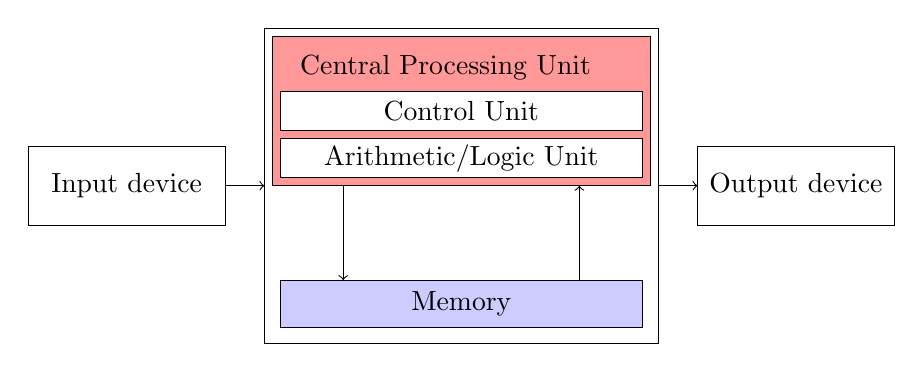
\begin{tikzpicture}
	\draw (3,0) rectangle (8,4);
	\draw (3.1,2) [fill=red!40] rectangle (7.9,3.9);
	\node at (5.3,3.5) {Central Processing Unit};

	\draw (3.2,2.1) [fill=white] rectangle (7.8,2.6) node[pos=.5] {Arithmetic/Logic Unit};
	\draw (3.2,2.7) [fill=white] rectangle (7.8,3.2) node[pos=.5] {Control Unit};

	\draw (0,1.5) rectangle (2.5,2.5) node[pos=.5] {Input device};
	\draw (8.5,1.5) rectangle (11,2.5) node[pos=.5] {Output device};
	\draw [->] (2.5,2) -- (3,2);
	\draw [->] (8,2) -- (8.5,2);

	\draw (3.2,.2) [fill=blue!20] rectangle (7.8,.8) node[pos=.5] {Memory};
	\draw [->] (4,2) -- (4,.8);
	\draw [->] (7,.8) -- (7,2);
\end{tikzpicture}
\caption{Von Neumann model}
\label{fig:1_HPC:von_neumann_model}
\end{figure}

On that figure we can identify several three parts, the input and output devices and in the middle the computational device itself. 
The input device and output device are used to store in a read/write way data. 
It can be represented by hard drives or solid state drives.
Inside the computational device we find the memory, for the most common nowadays architectures it can be considered as a Random Access Memory (RAM). 
Several kind of memory exists and will be discussed later. 
The Central Processing Unit, CPU, is composed of several elements in this model. 
On one hand, the Arithmetic and Logic Unit, ALU, which takes as input one or two values and apply an operation on those data. 
They can be either logics with operations such as AND, OR, XOR, etc. or arithmetique with operations such as ADD, MUL, SUB, etc.
On the other hand, the Control Unit, CU, which control the data carriage to the ALU from the memory and the operation to be perform on data.

This is the basic model, some representation add another layer in the CPU called Registers, to store the local data of the ALU and CU. 
Of course, the links between those elements are important and called Buses and can be separated between data buses, control buses and adresses buses. 

Every devices or machines we will describe in the next chapter will have the same architecture using a CPU or several of them with memory. 

\section{Flynn taxonomy and executions models}

The Von Neumann model gives us a generic idea of how a computational unit is fashioned. 
But the technology keep evoluating and, at some point in early twentieth century, IBM proposed the first multi-core processor on the same die, the Power4.
in addition to the classical model, several arrangements are possible between the computational cores and the data to handle. 

A right characterization is then essential to be able to target the right architecture for the right purpose. 
The flynn taxonomy presents a hierarchical organization of computation machine and executions models.
In this classification~\cite{flynn1972some}, Michael J. Flynn present the SIMD, SISI, MISD and MIMD models.

\begin{center}
\[\arraycolsep=1.4pt\def\arraystretch{2.2}
\begin{tabular}{| l | l | l |}
\hline
Instructions / Data	& Single Data (SD) 	& Multiple Data (MD) \\
\hline
Single Instruction (SI)		&  SISD			& SIMD \\
\hline
Multiple Instructions (MI) 	& 	MISD		& MIMD \\
\hline
\end{tabular}
\]
\end{center}

\subsection{Single Instruction, Single Data: SISD}
This is the model corresponding to a single core CPU with no data parallelism. 
This sequential model is one instruction operate on one data which is then store and the process continue over. 
SISD is important to consider and can dominate the execution time due to the Amdahl's law, describe in next part. 

\subsection{Single Instruction, Multiple Data: SIMD}
This is the execution model corresponding to a many-core architecture like a GPU. 
In the same clock, the same operation is executed on every process on different data. 
The best example stay the work on matrices like a stencil. 
SIMD can be extended from 2 to 16 elements for classical CPUs to hundreds and even thousands of core for GPGPUs. 

\subsection{Multiple Instructions, Multiple Data: MIMD}
Every element executes its own instructions on its own data set. 
This can represent the behavior of a CPU using several cores, threads or even the differents nodes of a supercomputer cluster. 

\subsection{Multiple Instructions, Single Data: MISD}
This last model can correspond to a pipeline representation but even in this case the data are modified after every operations. 

We can also find another characterization to describe the new GPUs architecture: Single Instruction, Multiple Threads. 
This appears in NVIDIA's paper~\cite{lindholm2008nvidia}. 
This model describes a stack of SIMD architectures, every block of threads is working with the same control processor on different data. 
This is the model we describe in next chapter used for the \textit{warps} in NVIDIA CUDA.

\section{Memory}
In addition of the computational model and parallelism, multi-threading, the memory accesses parterns have a main role on performances. 

Different memory technologies exists and the aim is always greater capacity, better speed and bandwidth.

\subsection{Memory technologies}

\todo{Hard drives ??}

\subsubsection{SRAM}
The Static Random Access Memory is built using and is mainly used for cache memory. 
Based on commonly called "flip-flop" circuits that can store the data as long as the machine is powered. 
This kind of memory is very expensive to produice and is usually limited for small amount of storage. 

\subsubsection{DRAM}
The Dynamic Random Access Memory, at the opposite to the SRAM, is based on transistors to store the binary information.
This memory is less expansive to produice but needs to be refresh at a determined time however the data are lost. 
There is several sub categories of DRAM used in different devices. 

Depending on the way the bus are used we can find Single Data Rate, SDR, Double Data Rate, DDR and QDR, Quad Data Rates DRAM memories. 
The number of data carried can go from 1x to 4x but the limitation of those products is the price of memory constantly rising. 

We can also find Error-Correcting Code, ECC, memory which implements a bunch of data correction algorithm be garanty the validity of them when error is not allowed. 


\subsection{Shared memory}
In case of the SISD the memory access is just serial and no really rules needs to be set for its usage. 
When it comes to multi-threaded and multi-cores approaches several kind of memory can be used. 
We give a description of the most common shared memories architecures. 

\hspace*{-2cm}
\begin{figure}
\centering 
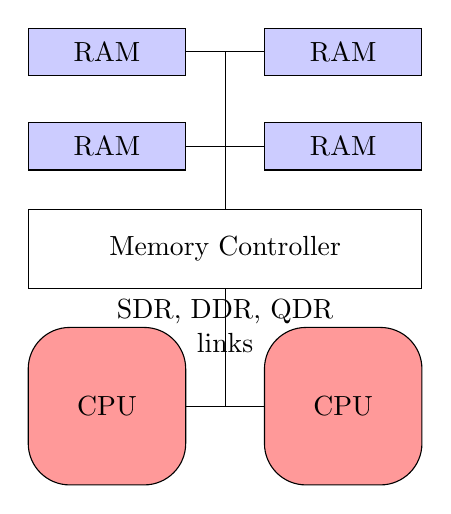
\begin{tikzpicture}
	\draw [rounded corners=15pt,fill=red!40] (0,0) rectangle (2,2) node[pos=.5] {CPU};
	\draw [rounded corners=15pt,fill=red!40] (3,0) rectangle (5,2) node[pos=.5] {CPU};

	\draw (0,2.5) rectangle (5,3.5) node[pos=.5] {Memory Controller};

	\draw (0,4) [fill=blue!20] rectangle (2,4.6) node[pos=.5] {RAM};
	\draw (0,5.2) [fill=blue!20] rectangle (2,5.8) node[pos=.5] {RAM};
	
	\draw (3,4) [fill=blue!20] rectangle (5,4.6) node[pos=.5] {RAM};
	\draw (3,5.2) [fill=blue!20] rectangle (5,5.8) node[pos=.5] {RAM};

	\draw [-] (2,1) -- (3,1);
	\draw [-] (2.5,1) -- (2.5,2.5);
	\node at (2.5,2.2) {SDR, DDR, QDR};
	\node at (2.5,1.8) {links};

	\draw [-] (2.5,3.5) -- (2.5,5.5);
	\draw [-] (2,4.3) -- (3,4.3);
	\draw [-] (2,5.5) -- (3,5.5);
\end{tikzpicture}
\hspace{1cm}
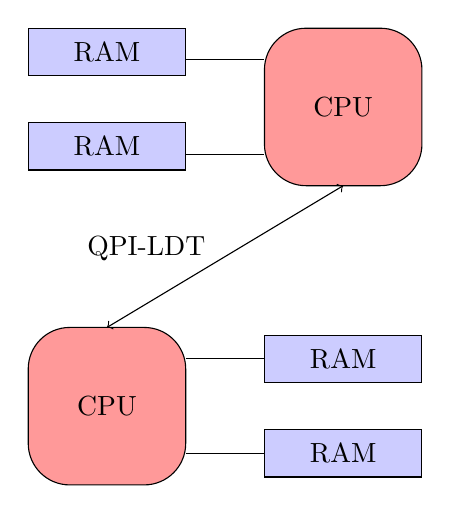
\begin{tikzpicture}
	\draw [rounded corners=15pt,fill=red!40] (0,0) rectangle (2,2) node[pos=.5] {CPU};
	\draw (3,0.1) [fill=blue!20] rectangle (5,0.7) node[pos=.5] {RAM};
	\draw (3,1.3) [fill=blue!20] rectangle (5,1.9) node[pos=.5] {RAM};
	\draw [-] (2,0.4) -- (3,0.4);
	\draw [-] (2,1.6) -- (3,1.6);
 	
	\draw [rounded corners=15pt,fill=red!40] (3,3.8) rectangle (5,5.8) node[pos=.5] {CPU};
	\draw (0,4) [fill=blue!20] rectangle (2,4.6) node[pos=.5] {RAM};
	\draw (0,5.2) [fill=blue!20] rectangle (2,5.8) node[pos=.5] {RAM};
	\draw [-] (2,4.2) -- (3,4.2);
	\draw [-] (2,5.4) -- (3,5.4);

	\draw [<->] (1,2) -- (4,3.8);
	\node at (1.5,3) {QPI-LDT};
\end{tikzpicture}
%\hspace{1cm}
%\begin{tikzpicture}
%	\draw [rounded corners=15pt] (1,0) rectangle (3,2) node[pos=.5] {CPU};
%	\draw [rounded corners=15pt] (1,3.8) rectangle (3,5.8) node[pos=.5] {CPU};
%
%	\draw (0,2.1) rectangle (2,2.8) node[pos=.5] {RAM};
%	\draw (0,3.2) rectangle (2,3.8) node[pos=.5] {RAM};
%	
%	\draw (3,2.2) rectangle (5,2.8) node[pos=.5] {RAM};
%	\draw (3,2.2) rectangle (5,3.8) node[pos=.5] {RAM};
%
%\end{tikzpicture}
\caption{UMA vs NUMA}
\label{fig:1_HPC:von_neumann_model}
\end{figure}

\subsubsection{UMA}
The Uniform Memory Access is a global memory shared by every threads or cores. 
In UMA every processors us its own cache as local memory. 
The addresses can be accessed directly by each processors. 

With the arising of accelerators like GPUs and their own memory, some constructors found ways to create UMA with heterogeneous memory. 
AMD creates the heterogeneous UMA, hUMA~\cite{rogers2013amd}, in 2013 allowing CPU and GPU to target the same memory area.

\subsubsection{NUMA}

In Non Unified Memory Access every processor have access to its own memory but allows other processors to access those area though Lightning Data Transport, LDT or Quick Path Interconnect, QPI, for Intel architectures. 

\todo{Present CC-NUMA and NC-NUMA.}

\subsubsection{COMA}
In Cache-Only Memory Accesses, the whole memory is see as a cache from every processes.
Attraction memory is setting up and will attract the data near the process that will use those data. 
This model is less commonly use and lead to, at best, same results as NUMA.

\section{Speedup, efficiency and scalability}

In the previous parts we described the differents models, characterizations and memory patterns for HPC. 
Based on those tools we need to be able to emphasis the performances of a computer and supercomputer. 

\subsection{Speedup and efficiency}
Calling latency the time to computer a time, unit of time. 
The latency is define as the time for number
The lower latency is better. 

Considering $n$ the number of processes and $n=1$ the sequential case.
And $T_n$ the execution time with $n$ processes and $T_1$ the sequential one. 
The speedup can be defined using the latency by the formula: 
\begin{equation}
\text{speedup} = S_n =  \frac{T_1}{T_n}
\end{equation}


\begin{figure}
\centering 
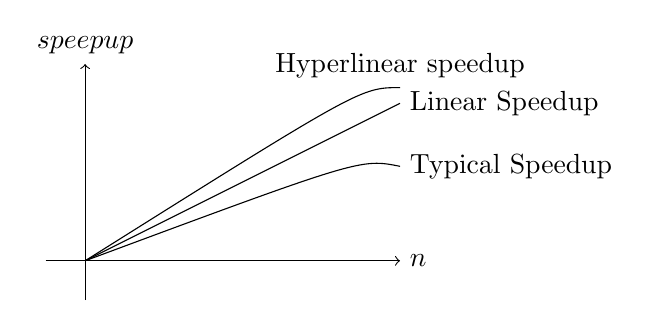
\begin{tikzpicture}
  \draw[->] (-.5,0) -- (4,0) node[right] {$n$};
  \draw[->] (0,-.5) -- (0,2.5) node[above] {$speepup$};
  \draw (0,0) -- (4,2) node[right] {\text{Linear Speedup}};
  \draw (0,0) .. controls (3.5,1.3) .. (4.,1.2) node[right] {\text{Typical Speedup}} ;
  \draw (0,0) .. controls (3.5,2.2) .. (4.,2.2) node[above] {\text{Hyperlinear speedup}} ;
\end{tikzpicture}
\caption{Observed speedup}
\label{fig:1_HPC:speedup_obs}
\end{figure}

As shown on figure \ref{fig:1_HPC:speedup_obs} several kind of speedup can be observed. 
\paragraph{Linear}
The linear speedup usually represent the target for every programs in HPC. 
Indeed having the speedup growing exactly as the number of processors grows is the ideal case. 
Codes fall typical into two cases. 
\paragraph{Typical speedup}
This represents the most common observed speedup. 
As the number of processors grows, the program face several of the HPC walls, the hardest being communications.
So the increasing number of computational power is reduiced to the sequential pqrt or lose time in exchanges. 
\paragraph{Hyperlinear speedup}
In some cases we can observe an hyperlinear speedup, meaning that the results in parallel are even better than the ideal case. 
Several explainations can be given. 
The program can fit exactly in memory for less data on each processors or even fir perfectly for the cache utilization. 
The parallel algorithm can also be way more efficient than the sequential one. 

And the efficiency is defined by the speedup devided by the number of workers: 
\begin{equation}
\text{efficiency} = \frac{S_n}{n} = \frac{T_1}{nT_n}
\end{equation}

The efficiency, usually expressed in percent, represent the evolution of the code stability to growing number of processors. 


\subsection{Scalability}

\section{Amdhal's and Gustafson's law}

The Amdhal's and Gustafson's law show us how to be able to evaluate the maximal available speedup for an application taking in account different characteristics. 

\subsection{Amdahl's law}

The Amdahl's law\cite{amdahl1967validity} is use to find the theoretical speedup in latency of a program.
We can separate a program in two parts, the one that can be execute in parallel and the one that is sequential. 
And even if we reduce the parallel part to infinite the sequential part will reach 100\% of the total time. 

Extracted from the Amdahl paper the law can be writen as: 

\begin{equation}
Speedup = \frac{1}{Seq + \frac{Par}{n}}
\end{equation}

Where $Seq + Par = 1$ and $Seq$ and $Par$ respectively the sequential and parallel ratio of a program.

This is also called strong scaling.  

And the efficiency become:
\begin{equation}
Efficiency = \frac{n}{Seq + \frac{Par}{n}}
\end{equation}

\subsection{Gustafson's law}

The Amdhal's law is focused on problem with the same memory size. 
John L. Gustafson's idea is that using more computational units, the problem size can grow accordingly. 
He considered a constant computation time with evolving problem size. 
With this point of view using more computational units leads to better results 

The speedup:
\begin{equation}
Speedup = Seq + Par \times n
\end{equation}

\section{Conclusions}

In this chapter we presented the different basic tools to be able to understand HPC. 
The Von Neumann model that represent every nowadays architecture. 
The Flynn taxonomy that is in constant evolution with new paradigms like recent SIMT from NVIDIA. 
We also presented the memory types that will be use at different layers in our clusters, from node memory, CPU-GPGPU shared memory space to global fast shared memory. 
We finished by presenting the most important laws with Amdahl's and Gustafson's laws.
We introduice the concept of Strong and Weak scaling that will lead our tests through all the examples in Part II and Part III. 


%%%%%%%%%%%%%%%%%%%%%%%%%%%%%%%%%%%%%%%%%%%%%%%%%%%%%%%%%%%%%%%%%%%%%
%																	%
%	CHAPTER TWO, HARDWARE IN HPV									%
%																	%
%%%%%%%%%%%%%%%%%%%%%%%%%%%%%%%%%%%%%%%%%%%%%%%%%%%%%%%%%%%%%%%%%%%%%
\chapter{Hardware in HPC}

\section{Introduction}

Optimization can't be done without a good knowledge of the machine architecture. 
Indeed, nowaday software and API try to take care of most of the cases but the last percent of gain have to be architecture dependent. 
In this chapter we will describe the most important devices architecures from classical Central Processing Units (CPUs), General Purpose Graphics Processing Units (GPGPUs), Field Programmable Gate Arrays (FPGAs) and Application-specific integrated circuits (ASICs).
Then those independants elements are use together in order to build supercomputers. 
The way they are arranged and the nodes interconnection is something that really matter at large scale.  

\section{Architectures}
\subsection{Classical CPU}

The CPU, as we know it today, begin its history with \textit{Texas Instruments Inc} and the first patent describing a CPU is "Computing systems cpu" proposed by \textit{Gary Boone} and published in 1973.
This first fonctional processing unit on chip and is based on the Von Neumann Model.
Before that vacuum tubes were used instead of transistors making the space used very high.

The Von Neumann model can be extracted for the first time by the physists John Von Neumann and its team in \cite{} 
The Electric Discrete Variable Automatic Computer (EDVAC) presented in this paper was one of the first binary computer built with vacuum tubes. Von Neumann came in the project and summarized the logical aspects of this machine. 
This model is presented on Fig.~\ref{}.
since, every devices can be represented based on that model with optimizations in term of number of cores, memory accesses and bus. 




Talk about the ARM architecture 

\subsection{GPGPU}

GPUs are based on the SIMD model of the Flynn taxonomy presented previously, \emph{Single Instruction, Multiple Data}.
The specific execution model is called SIMT (\emph{Single Instruction, Multiple Thread}). It enables the execution of millions of coordinated threads in a data-parallel mode. 
Two main companies provide GPGPUs for the HPC world NVIDIA and AMD, we will present them in that order and conclude on the differences. 

\subsubsection{NVIDIA GPU architecture}

The NVIDIA company was fonded in April 1993 in Santa Clara, Carolina, by three persons in which Jensen Huang, the actual CEO.
Its name seems to come from \textit{invidia} the latin word for Envy and vision, for the graphics generation. 

Known as the pioner in graphics, cryptocurrency, portable devices and now AI, it seems to be even the creator of the name "GPU".
It GPU, inspired from visualisation and gaming at a first glance, is available as a dedicated device  since the Tesla. 
The public GPUs can also be use for dedicated computation but does not feature eMMC memory, double precision or special functions/FFT cores. 

We will describe here the Kepler architecture, this is the one we worked

\begin{figure*}[t!]
\centering
\setlength\fboxsep{0pt}
\setlength\fboxrule{0.25pt}
\includegraphics[scale=0.6]{figures/chap1/smx}
\caption{NVIDIA GPU and CUDA architecture overview}
 \label{fig:chap1_gpu}
%\vspace{-0.8cm} 
\end{figure*}

As presented in Fig.\ref{fig:chap1_gpu}, NVIDIA GPUs include many \emph{Streaming Multiprocessors} (SM), each of which is composed of many \emph{Streaming Processors} (SP). In the Kepler architecture, the SM new generation is called SMX.
%
%In the CUDA programing model~\cite{cuda}, the GPU works as a SIMT co-processor of a conventional CPU. 
Grouped into \emph{blocks}, \textit{threads} execute \emph{kernel} functions synchronously.
Threads within a block can cooperate by sharing data on an SMX and synchronizing their execution to coordinate memory accesses; inside a block, the scheduler organizes \emph{warps} of 32 threads which execute the instructions simultaneously.
The blocks are distributed over the GPU SMXs to be executed independently.

\subsubsection{Memory, bandwidth and streams:}

In order to use data in a CUDA kernel, it has to be first created on the CPU, allocated on the GPU and then transferred from the CPU to the GPU; after the kernel execution, the results have to be transferred back from the GPU to the CPU. 
GPUs consist of several memory categories, organized hierarchically and differing by size, bandwidth and latency.   
On the one hand, the device's main memory is relatively large but has a slow access time due to a huge latency. 
On the other hand, each SMX has a small amount of shared memory and L1 cache, accessible by its SPs, with faster access, and registers organized as an SP-local memory. 
SMXs also have a constant memory cache and a texture memory cache.
%, that are linked to the constant and texture memories physically located in the device memory: these are read-only and have faster access time than the rest of the memory categories.
Reaching optimal computing efficiency requires considerable effort while programming.
Most of the global memory latency can then be hidden by the threads scheduler if there is enough computational effort to be executed while waiting for the global memory access to complete. Another way to hide this latency is to use streams to overlap kernel computation and memory load. 

\subsubsection{Threads synchronization:}
It is also important to note that branching instructions may break the threads synchronous execution inside a warp and thus affect the program efficiency. 
This is the reason why test-based applications, like combinatorial problems that are inherently irregular, are considered as bad candidates for GPU implementation. 
%This is particularly true with regard to combinatorial problems resolution. 
Thus we intend to provide a way to regularize their execution, in order to get good acceleration with GPU computation. 

\subsubsection{Details on K20Xm}

\todo{Describe K20Xm, 2688 cores}

\subsection{FPGA and ASICS}

\section{Clusters and interconnection}
\subsection{TOP500 remarquable clusters}
\subsubsection{Sunway Taihulight}

Sunway Taihulight is the third Chinese supercomputer to be ranked in the first position of the TOP500 list. \todo{(VERIFIER)}
A recent report from Jack Dongarra, a figure in HPC, decrypt the architecture of this supercomputer\cite{dongarra2016report}. 
The most interessant point is the conception of this machine, completely done in China. 
The Sunway CPUs were invented and built in China, the Vendor is the Shanghai High Performance IC Design Center. 

\begin{figure}
\centering
\includegraphics[scale=1]{figures/Chap1/report_sunway_CPE}
\caption{Sunway Taihulight node architecture from \textit{Report on the Sunway TaihuLight System}, Jack Dongarra, June 24, 2016.}
\label{fig:chap1_report_sunway_CPE}
\end{figure}

The SW26010, a many core architecture, features 260 cores based on RISC architecture and a specific conception depicted on Fig.\ref{fig:chap1_report_sunway_CPE}.


\subsubsection{Titan}
\subsubsection{K-Computer}
\subsubsection{Sequoia}
\section{ROMEO Supercomputer}

The ROMEO supercomputer center is the computation center of the Champagne-Ardenne region in France. 
Hosted since 2002 by the University of Reims Champagne-Ardenne, this so called meso-center (French name for software and hardware architectures) is used for HPC for theoric research and domain science like applied mathematics, physics, biophysics and chemistry. 

This project is support by the Champagne-Ardenne region and the CEA (French Alternative Energies and Atomic Energy Commission), aim to host research and production codes of the region for industrial, research and academics purposes. 

We are currently working on the third version of ROMEO, installed in 2013. 
As many of our tests in this study have been done on this machine, we will carefully describe its architecture. 

This supercomputer was ranked 151st in the TOP500 and 5th in the GREEN500 list. 

\subsection{ROMEO hardware architecture}
ROMEO is a Bull/Atos supercomputer composed of 130 BullX R421 computing nodes. 

Each node is composed of two processors Intel Ivy Bridge 8 coeurs @ 2,6 GHz. 
Each processor have access to 16GB of memory for a total of 32GB per node, the total memory if 4.160TB. 
Each processor if linked, using PCIe-v3, to an NVIDIA Tesla K20Xm GPGPU. 
This cluster provide then 260 processors for a total of 2080 CPU cores and 260 GPGPU providing 698880 GPU cores. 
The computation nodes are interconnected with an Infiniband QDR non-blocking network structured as a FatTree. 
The Infiniband is a QDR providing 10GB/s. 

The storage for users is 57 TB and the cluster also provide 195 GB of Lustre and 88TB of parallel scratch filesystem. 

In addition to the 130 computations nodes, the cluster provides a visualization node NVIDIA GRID with two K2 cards and 250GB of DDR3 RAM. 
The old machine, renamed Clovis, is always available but does not features GPUs. 

The supercomputer supports MPI with GPU Aware and GPUDirect. 

%%%%%%%%%%%%%%%%%%%%%%%%%%%%%%%%%%%%%%%%%%%%%%%%%%%%%%%%%%%%%%%%%%%%%
%																	%
%	CHAPTER THREE, SOFTWARE AND API									%
%																	%
%%%%%%%%%%%%%%%%%%%%%%%%%%%%%%%%%%%%%%%%%%%%%%%%%%%%%%%%%%%%%%%%%%%%%
\chapter{Software and Benchmarks}

\section{Sofware/API}
\subsection{OpenMP}
\subsection{MPI}
\subsection{CUDA}
\subsection{Charm++}
\subsection{Legion}
\section{Benchmark}
\subsection{TOP500}
\subsection{GRAPH500}
\subsection{GRENN500}

\chapter*{Conclusion}

% Chapter Two 
\chapter{Complex systems}

\section{Introduction}

\section{Combinatorial problems}

\subsection{Combinatorial search}

\subsection{Combinatorial optimization}

\section{A case study, the Langford problem}

Use the articles here for figures and a base report. 
 
\section{Complex systems as a benchmark} 

\section{GRAPH500}

Use the articles here too 
 
\section{Conclusion}
% Chapter Three 
\input{chapters/3_application}
% Conclusion
\addcontentsline{toc}{chapter}{Conclusion}
\chapter*{Conclusion}
The first part of this study described the tools and theories needed to understand and reach performances in HPC. 
We presented several architectures and their advantages and showed the next objective for the world most powerful countries is to reach the computational power of one exaflop by the year 2020. 
Our belief is that these architectures will be hybrid powered by accelerators with many-cores, such as GPU or FPGAs. \\

We defined a metric targeting the most important walls of HPC from this observation regarding the power consumption and computation performances.
The intent of this metric was to confront classical and hybrid architecture to show the real benefit that can be obtained by using accelerators. 
This metric is separated in two parts. 

In the fist part, we targeted classical, academical and even benchmark problems as the metric. 
We compared the classical architecture to a hybrid counterpart using on a problem featuring heavy computation and a second one focusing heavy communications. 
In both cases, we wanted to fit production code and their worst behavior: irregularity. 

The first problem was the Langford pairing counting problem. 
This problem was studied with two different approaches based on a tree traversal and an arithmetic resolution, respectively. 
The tree resolution showed very good results and up to 80\% of the overall work handle by the GPU with an efficient load balancing strategy. 
The mathematical solution was also very irregular due to the large integer arithmetic on GPUs. 
In this case, we showed that the GPU was able to handle up to 65\% of the computation effort. 
This hybrid architecture implementation allowed us to beat a timed record for the computation of the last instances using best-effort on the ROMEO supercomputer. 

The second problem we addressed was the Graph500 benchmark. 
This was a perfect candidate in order to consider communication problems without heavy computation. 
Indeed, the only operations needed were memory checking for values and copies in queues. 
This problem stayed very irregular in both the memory and the communication usage. 
We proposed an algorithm based on both NVIDIA and IBM BlueGene/Q state of the art algorithm. 
This allowed us to rank the ROMEO supercomputer 105th in the November 2016 Graph500 list.
This metric showed the high level of scalability that can be reach with GPUs.\\

These two first approaches gave a lot of credit to the hybrid architecture on both walls separately. 
In order to complete our metric we needed to examine the classical and hybrid architectures to a production application issuing both walls. 
We targeted a complex simulation application. 
The problem fitting our needs in computational and communication over irregular context was the smoothed particle hydrodynamics and gravitation simulation of hard astrophysics events. 
We developed, in collaboration with the Los Alamos National Laboratory, a framework named FleCSPH dedicated to tree topology and physics/astrophysics simulations. 
We showed with this metric the performances using hybrid architectures. 
Even keeping an approach of production code, not fully GPU, the performances on hybrid architectures can be greatly superior to classical CPU ones. 

This study showed three base cases where the hybrid architecture can be the solution for exascale supercomputer.
The main walls are solved using generic strategies and new ways of thinking about the algorithms. \\

Hybrid architectures appears to be the approach for building Exascale supercomputers but computer science is a very fast evolving field of research.  
The release of a new technologies can change the cards and lead to better, alternative solutions.
The main proposal, beside classical architectures and hybrid ones, is the ARM powered supercomputers. 
We presented the Montblanc project, the European effort to reach exascale with reduce instruction set processors enabling low energy consumption. 
Other groups are also interested in this type of ARM architecture. 
The Japanese supercomputer center, K computer with RIKEN, is known to integrate a very efficient interconnect with a 6 dimensional torus.
The next generation of this project, the post-K\footnote{http://www.fujitsu.com/global/Images/post-k-supercomputer-overview.pdf} computer, will keep the same TOFU interconnection topology, but provide ARMv8 processors. 

Currently, another solution for specific problems seems to be resolved in so called Quantum Computing.
The \textit{bits} of classical processors are replaced by \textit{qubits}, quantum bits, and can provide more states than the usual 0 - 1 of bits.
These specific machines are based on probabilities and seem to target very specific applications. 
Quantum Computers are always in development but some center, like the ROMEO supercomputer center, provide simulation of quantum computers behavior in order to learn their utilizations.\\

The evolution of hardware will lead to bigger and more complex supercomputers. 
Computer scientists need to reconsider new ways to think of algorithms and implementation. 
On one hand, the tools like API and framework have to be able to target all the architecture and topologies.
On the other hand, algorithms have to be think natively for massive parallel architecture and most of the existing ones changed.
As an example, stochastic approaches can a way to reach a result faster with an error determined by the user, perfect for computations based on Montecarlo or current fields, such as AI. 


% Annexes
`\addcontentsline{toc}{chapter}{Annexes}
\input{chapters/annexes}


% Bibliography
\addcontentsline{toc}{chapter}{Bibliography}
\bibliographystyle{alpha}
\nocite{*}
\bibliography{biblio/biblio_langford,biblio/biblio_graph,biblio/biblio_sph,biblio/biblio_misc}

\end{document}